%class
	\documentclass{beamer}

%template
	\usetheme{HannoverSalman}
	\setbeamertemplate{navigation symbols}{}
	%\setbeamertemplate{footline}{\centering{\insertframenumber/\insertpresentationendpage}}
	%\setbeamertemplate{footline}{\hspace*{.5cm}\scriptsize{\hfill\insertframenumber\hspace*{.5cm}}} 


%packages
	\usepackage{amsmath, amssymb, graphicx,cancel}
	\usepackage[absolute,overlay]{textpos}
	\usepackage{subfigure}
	\usepackage{caption}\captionsetup{labelformat=empty,labelsep=none}
	\usepackage{geometry}
	\geometry{verbose}
	\usepackage{color}
	\usepackage{xmpmulti}
	\usepackage[3D]{movie15}
	\usepackage{hyperref}
%	\usepackage{bookmark}
	\usepackage[open,openlevel=4,atend]{bookmark}
	%\bookmarksetup{color=blue}
	\usepackage{multirow}
	\usepackage[style=numeric,defernumbers, authoryear]{biblatex}
	%\usepackage[square,sort]{natbib}
	%\usepackage{fancyhdr}%\pagestyle{fancy} 

	
	\hypersetup{bookmarksdepth = 4}


%citations files
	\bibliography{MyCitations}

%logoCSIPCPL
    \setlength{\TPHorizModule}{1mm}
    \setlength{\TPVertModule}{1mm}
    \newcommand{\logoCSIPCPL}
    {
    	\begin{textblock}{1}(100,2) %(100,85)  for bottom
    		
\includegraphics[width=1.5cm]{figs/logo_CSIP}
    	\end{textblock}
    	
	\begin{textblock}{1}(117,1) %(117,85)  for bottom
    		
\includegraphics[width=1.0cm]{figs/logo_CPL}
    	\end{textblock} 
    }

%logo evolution
    \newcommand{\logoEvolution}
    {    	
	\begin{textblock}{1}(110,1) %(117,85)  for bottom
    		\includegraphics[width=0.65in]{figs/logo_evolution.pdf}
    	\end{textblock} 
    }

%logo Qualcomm
    \newcommand{\logoQualcomm}
    {
    	\begin{textblock}{1}(110,2) %(100,85)  for bottom
    		\includegraphics[width=1.5cm]{figs/logo_qualcomm.jpg}
    	\end{textblock}
    }
%logo Qualcomm (long)
    \newcommand{\logoQualcommllong}
    {
    	\begin{textblock}{1}(0,0) 
    		\includegraphics[width=1.25in]{figs/logo_qualcomm_long.jpg}
    	\end{textblock}
    }

%logo Tech Tower
    \newcommand{\logoTechTower}
    {
    	\begin{textblock}{1}(0,0) 
    		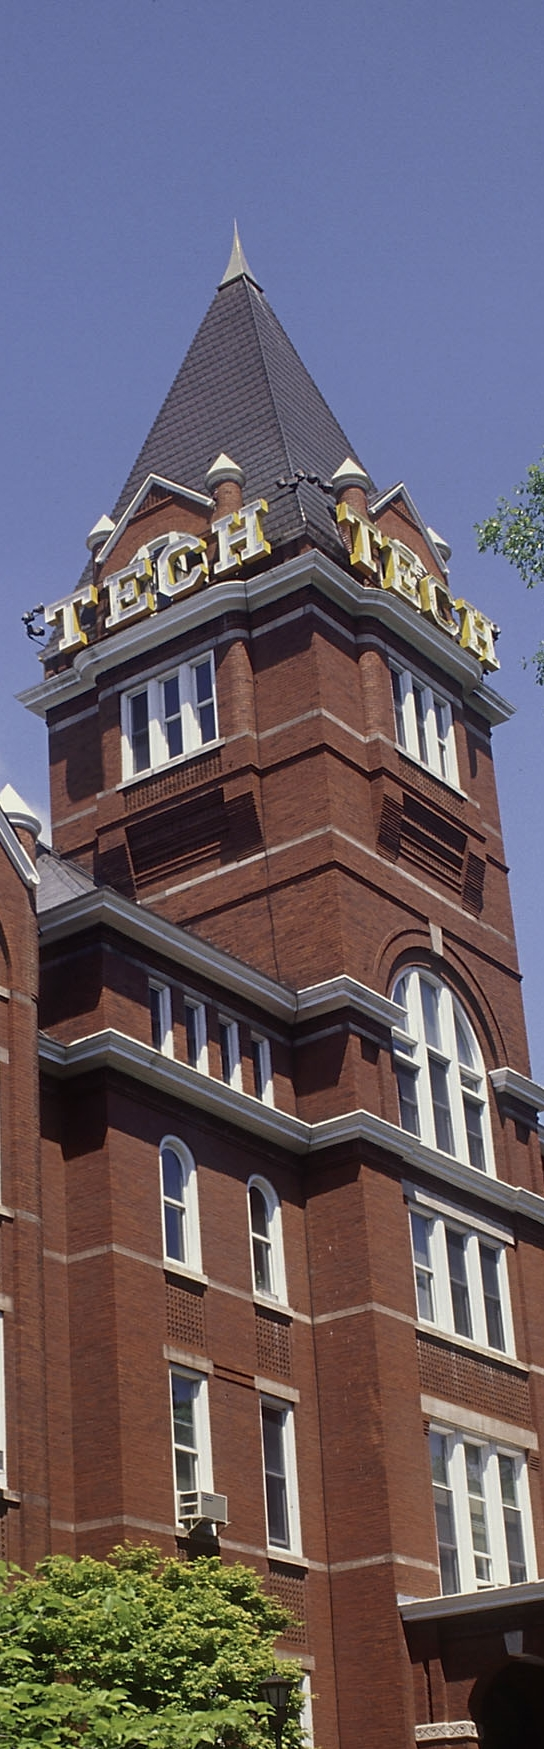
\includegraphics[width=1.25in]{figs/logo_TechTower.jpg}
    	\end{textblock}
    }

%logo tree
    \newcommand{\logoTree}
    {
    	\begin{textblock}{1}(0,0) 
    		\includegraphics[width=1.25in]{figs/logo_tree.jpg}
    	\end{textblock}
    }
%page numbers
    \newcommand{\mypagenum}
    {
    	\begin{textblock}{1}(1,94) 
		{\tiny \color[rgb]{0.2,0.2,1}\insertframenumber} %\insertframenumber,\insertpresentationendpage, \inserttotalframenumber
    	\end{textblock}
    }
%my footnote citation
	\newcommand{\myFootnoteCitation}[2]
	{
		\footnote{\tiny \citeauthor{#1}, \emph{#2}, \citeyear{#1}.}  %\citeauthor{#1}, \citetitle{#1}, #2 \citeyear{#1}.
	}
%my refer to citation
	\newcommand{\mycite}[1]
	{
		\emph{\citeauthor{#1} (\citeyear{#1})}
	}
%my footnote website citation
	\newcommand{\myFootnoteWebsiteCitation}[1]
	{
		\footnote{\tiny \citeauthor{#1}}
	}

\let\thefootnote\relax\footnotetext{Footnotetext without footnote mark}


%section underline
%\newcommand{\tmpsection}[1]{}
%\let\tmpsection=\section
%\renewcommand{\section}[1]{\tmpsection{\underline{#1}}}



%commands
	\newcommand{\likelihood}{p(Z_k| x_k) }						%likelihood
	\newcommand{\prior}{p(x_k)  } 								%prior
	\newcommand{\posterior} {p(x_k| Z_k)}						%posterior
	\newcommand{\prediction} {p(x_k| Z_{k-1})}					%prediction
	\newcommand{\update} {p(x_k|Z_k)}							%update
	\newcommand{\observations} {p(Z_k)}						%observations
	\newcommand{\prevobservations} {p(Z_{k-1})}				%previous observations
	\newcommand{\dxpk} {dx_{k-1}}							%dx_{k-1}
	\newcommand{\ChapKolm}{\int{p(x_k| x_{k-1})p(x_{k-1}|Z_{k-1})} \dxpk} %Chapman Kolmogorov

	%algorithm specific: JPDAF
	\newcommand{\likelihoodJPDAF}{p(Z_k| \chi, m, Z_{k-1}) }		%1. likelihood
	\newcommand{\priorJPDAF}{p(\chi|m, Z^{k-1}} 				%2. prior	
	\newcommand{\observationsJPDAF} {p(Z_k}					%3. observations
	\newcommand{\posteriorJPDAF} {p(\chi| Z_k)}					%4. posterior

%environments
	\newenvironment{changemargin}[2]
	{
	  	\begin{list}{}
		{
			\setlength{\topsep}{0pt}%
			\setlength{\leftmargin}{#1}%
			\setlength{\rightmargin}{#2}%
			\setlength{\listparindent}{\parindent}%
			\setlength{\itemindent}{\parindent}%
			\setlength{\parsep}{\parskip}%
		}
	  	\item[]
		}
		{\end{list}
	}
%figures

%colors
\definecolor{darkgreen}{rgb}{0,0.5,0}

%personal details
	\author{Salman Aslam}
	\institute{Advisor, Dr Christopher Barnes (ECE)\\Co-advisor, Dr Aaron Bobick (CoC)\\Georgia Institute of Technology}
	\date{}

\begin{document}
%####################################################################################################
\title{Programming}
%####################################################################################################
\begin{frame}\logoTree
	\institute{}
	\titlepage
\end{frame}

\begin{frame}\frametitle{Outline}\logoTree
	\setcounter{tocdepth}{1}	
	\tableofcontents
\end{frame}




%#######################################################################
\section{Introduction}
%#######################################################################
\begin{frame}[plain]\logoEvolution\mypagenum
	\begin{changemargin}{-1.3in}{0in}
		\begin{figure}
			\includegraphics[width=1.3\textwidth]{figs/GPU_history_of_HPC}
		\end{figure}	
	\end{changemargin}
\end{frame}



\begin{frame}\frametitle{History (cont.)}\logoEvolution\mypagenum
	\begin{itemize}
	\item GPU implementations, originally low-level %\cite{2007_CNF_OpticalFlowCUDA_Mizukami}
		\begin{itemize}
			\item 2002: \emph{Cg}
			\item 2004: \emph{HLSL}
			\item Knowledge of computer graphics required
			\item Learning curve
		\end{itemize}
	\item Nvidia CUDA, 2007
		\begin{itemize}
			\item 1999: GPU invented
			\item Instruction set as an extension to \emph{C}
			\item Block: shared memory for threads, resides on chip
		\end{itemize}	
	\end{itemize}
\end{frame}


%#######################################################################
\section{C/C++}
%#######################################################################
%==============================
\subsection{Visual Studio tips}
%==============================
\begin{frame}
\frametitle{Visual Studio tips}
\framesubtitle{adding keywords for syntax highlighting}
\logoCSIPCPL\mypagenum	
	\begin{itemize}
		\item create usertype.dat in \textless Visual Studio Directory \textgreater  \textbackslash Common7 \textbackslash IDE
		\item put your keywords in that file, one per line
		\item some words: string CString CFile ULONGLONG ifstream ofstream byte FILE
	\end{itemize}
\end{frame}


\begin{frame}
\frametitle{Introduction}
\framesubtitle{environment variables}
\logoCSIPCPL\mypagenum
	\begin{itemize}\tiny	
		\item View -\textgreater Property Pages -\textgreater Configuration Properties -\textgreater  
			\begin{itemize}\tiny
				\item General -\textgreater Output directory, by default is \$(SolutionDir)\$(ConfigurationName)	
				\item General -\textgreater Intermediate directory by default is \$(ConfigurationName)
				\item Linker -\textgreater General -\textgreater Output file, by default is \$(OutDir)\textbackslash \$(ProjectName).exe	
			\end{itemize}
	\end{itemize}
\end{frame}



\begin{frame}
\frametitle{Introduction}
\framesubtitle{environment variables}
\logoCSIPCPL\mypagenum
	\begin{itemize}
		\item open memory windows to debug code
			\begin{itemize}
				\item press Ctrl-Alt-M together, leave, then press 1, 2, 3 or 4
			\end{itemize}
	\end{itemize}
\end{frame}




%==============================
\subsection{Strings}
%==============================
\begin{frame}
\frametitle{Strings}
\framesubtitle{}
\logoCSIPCPL\mypagenum
	\begin{block}{convert from char* to}
		\tiny
		{\color{blue}char}* stringC = "Hello, World!";{\color{green}// C}\\ 
		\vspace{0.1in}
		{\color{green}/*1*/}{\color{blue}std::string} stringCPP(stringC); {\color{green}// C++}\\
    		{\color{green}/*2*/}{\color{blue}CString} stringMFC(stringC);{\color{green}// MFC}\\
		{\color{green}/*3*/}{\color{blue}System::String}\^ \ stringDotNET = {\color{blue}gcnew System::String}(stringC); {\color{green}//.NET}\\
	\end{block}
	\vspace{0.2in}
	\begin{block}{convert from std::string to}
		\tiny
		{\color{blue}std::string} stringCPP = "Hello, World!";{\color{green}// C++}\\  
		\vspace{0.1in}
		{\color{green}/*1*/}{\color{blue}char}* stringC=stringCPP.c\_str(); {\color{green}// C}\\
    		{\color{green}/*2*/}MFC: same as above using stringCPP.c\_str()\\
		{\color{green}/*3*/}.NET: same as above using stringCPP.c\_str()\\
	\end{block}
\footnote{\tiny {\color{blue}  \href{http://msdn.microsoft.com/en-us/library/ms235631(VS.80).aspx}{http://msdn.microsoft.com/en-us/library/ms235631(VS.80).aspx}}}
\end{frame}


\begin{frame}
\frametitle{Strings}
\framesubtitle{}
\logoCSIPCPL\mypagenum
	\begin{block}{convert from CString to}
	\end{block}
	\vspace{0.2in}
	\begin{block}{convert from System::String\^ \ to}
	\end{block}
\footnote{\tiny {\color{blue}  \href{http://msdn.microsoft.com/en-us/library/ms235631(VS.80).aspx}{http://msdn.microsoft.com/en-us/library/ms235631(VS.80).aspx}}}
\end{frame}


%==============================
\subsection{Files}
%==============================
\begin{frame}[fragile]
\frametitle{Files}
\framesubtitle{read text file using fields}
\logoCSIPCPL\mypagenum
\tiny
\begin{verbatim}
int  main(void)
{
	std::string strLine;
	int intWidth, intHeight, intX, intY;
	string strField;
	string strFileName;
	int cnt;

	ifstream infile("TrainingFiles1.txt");
	while (!infile.eof())
	{
		//read line
		getline(infile, strLine);
		stringstream ssLine(strLine);	//string  ->stringstream ->string	 ->stringstream
										//strLine ->ssLine       ->strField  ->ssField
										//first stringstream  (ssLine)  helps in going from one string to another, i.e. line to field     
										//second stringstream (ssField) helps in converting a string to numbers, etc.
		cnt=1;

		//go over fields in line
		while (getline( ssLine, strField, ',' ))
		{
			stringstream ssField( strField );
			if		(cnt==1)	ssField>>strFileName;	
			else if (cnt==2)	ssField>>intWidth;
			else if (cnt==3)	ssField>>intHeight;
			else if (cnt==4)	ssField>>intX;
			else if (cnt==5)	ssField>>intY;
			
			cnt++;
		}
	}
	return 1;
}
\end{verbatim}
\end{frame}


\begin{frame}[fragile]
\frametitle{Files}
\framesubtitle{read one line of file into buffer}
\logoCSIPCPL\mypagenum
\tiny
\begin{verbatim}
#include <fstream>
#include <iostream>

std::ifstream in(filename.c_str());
if (!in.is_open())
	cerr << filename << ": tough luck!" << endl;

const int BUFSIZE = 10000;
char buf[BUFSIZE];
while (!in.eof())
{
    in.getline(buf, BUFSIZE-1);
}
\end{verbatim}
\end{frame}


\begin{frame}[fragile]
\frametitle{File}
\framesubtitle{read one line of file into buffer}
\logoCSIPCPL\mypagenum
\tiny
\begin{verbatim}
#include <fstream>
#include <iostream>

std::ifstream in(filename.c_str());
if (!in.is_open())
	cerr << filename << ": tough luck!" << endl;

in.read (buffer,length);
in.close();
\end{verbatim}
\end{frame}


\begin{frame}[fragile]
\frametitle{File}
\framesubtitle{MFC vs C++}
\logoCSIPCPL\mypagenum
\tiny
{\color{green}declarations}
\begin{verbatim}
CFile					cfile;
CFileException			fe;
ifstream				ifs;
ofstream				ofs;
char* buf  =	new char[numBytes];
\end{verbatim}
{\color{green}opening a file}
\begin{verbatim}
cfile.Open( charFileName, CFile::modeRead, &fe);
ifs.open(charFileName, ios::binary); if (ifs.is_open() cout<<"good");
\end{verbatim}
\tiny
{\color{green}read buffer from file}
\begin{verbatim}
cfile.Read(buf, numBytes);
ifs.read(buf, numBytes);
\end{verbatim}
\tiny
{\color{green}write buffer to file}
\begin{verbatim}
cfile.Write(buf, numBytes);
ofs.write(buf, numBytes);
\end{verbatim}
\tiny
{\color{green} close file}
\begin{verbatim}
cfile.Close();
ofs.close();
\end{verbatim}
\end{frame}


\begin{frame}[fragile]
\frametitle{g++}
\framesubtitle{}
\logoCSIPCPL\mypagenum
\tiny
\begin{verbatim}
a
\end{verbatim}
\end{frame}

%==============================
\subsection{Math}
%==============================
\begin{frame}[plain]
\frametitle{Math}
\framesubtitle{}
\logoCSIPCPL\mypagenum
\tiny
\begin{changemargin}{-1.43in}{0in}
\begin{tabular}{|l|l|l|}
\hline
C 						& Matlab 						& comments  \\ 
\hline
(int)x/(int)y 			& idivide(int32(x), int32(y)) 	& integer division\\
x\%y 					& mod(x,y) 					& remainder\\
\hline
floor(x) 				& same 						&\\
ceil(x) 					& same				 			&\\
floor(x+0.5) 			& round(x) 					&\\
\hline
\end{tabular}\\
I have a pixel, say (x,y) = (4,11) in C.  In Matlab it is (r,c) = (12,5), but for ease, let's say it is (5,12).  $I_w$ is image width\\
\begin{tabular}{|l|l|l|}
\hline
Operation 						& C 											& Matlab  \\ 
\hline
(x,y) $\rightarrow$ idx 		& $(y*I_w) + x = (11*640+4)=7044$ 		&  int32(((y-1)*$I_w$) + x)=int32(11*640+5)=7045\\
idx $\rightarrow$ y 			& (int)idx/(int)$I_w$=(int)7044/(int)640=11 	&  idivide(int32(idx), int32($I_w$), 'floor')+1=12\\
idx $\rightarrow$ x 			& idx \% $I_w$=7044\%640=4 				&  mod(int32(idx), int32($I_w$))=mod(int32(7045), int32(640))=5 \\
\hline
\end{tabular}\\
Matlab based indexing can have problems for values in the last columns\\
suppose you have a 3x4 matrix as follows:\\
    12    13    14    15\\
    17    18    19    20\\
    22    23    24    25\\
here the max index is 12 for the number 25.\\
using matlab based indexing, \\
y = idivide(int32(idx), int32($I_w$), 'floor')+1\\
x = mod(int32(idx), int32($I_w$))\\
gives me an index of [r,c]=[4,0]\\
therefore, best solution is that in Matlab, do idx-1, use C-style indexing to get x,y, then do x+1, y+1 to go back to Matlab-style indexing
\end{changemargin}
\end{frame}


%#######################################################################
\section{GPU}
%#######################################################################
\begin{frame}\frametitle{GPU vs CPU: speed}\logoEvolution\mypagenum
	\begin{itemize}
		\item GPU specialized for compute intensive, highly parallel computation
		\begin{figure}
			\includegraphics[width=3in]{figs/GPU_Intel_vs_Nvidia}
		\end{figure}
	\end{itemize}
\end{frame}



\begin{frame}\frametitle{GPU vs CPU: speed (cont.)}\logoEvolution\mypagenum
	\begin{itemize}
		\item Same program for each data element, so less flow control required
		\item Executed on many data elements, so access latency hidden with calculations rather than big data caches
		\begin{itemize}
			\item Designed for graphics rendering
		\end{itemize}
	\end{itemize}
\end{frame}




\begin{frame}\frametitle{GPU vs CPU: transistors}\logoEvolution\mypagenum
	\begin{itemize}
		\item GPU has high arithmetic intensity
		\begin{equation*}
			\text{Arithmetic \ intensity} = \frac{\text{arithmetic \ operations}}{\text{memory \ operations}}
		\end{equation*}
		\begin{figure}
			\includegraphics[width=3in]{figs/GPU_vs_CPU_transistors}
		\end{figure}
	\end{itemize}
\end{frame}





\begin{frame}\frametitle{Details}\logoEvolution\mypagenum
\end{frame}


\begin{frame}[plain]
	\begin{changemargin}{-1.3in}{0in}
		\begin{figure}
			\includegraphics[width=5in]{figs/GPU_SM.jpg}
		\end{figure}
	\end{changemargin}
\end{frame}




\begin{frame}\frametitle{Kernel}\logoEvolution\mypagenum
	\begin{itemize}
		\item C functions
		\item Called once, executed N times in parallel by N threads
		\item Number of threads is specified using $<<<...>>>$
	\end{itemize}
\end{frame}


\begin{frame}\frametitle{Threads}\logoEvolution\mypagenum
	\begin{itemize}
		\item Each thread has a unique ID, and is accessible through \textbf{threadIdx} variable
		\item \textbf{threadIdx} is a 3 component vector
		\begin{itemize}
			\item \textbf{threadIdx.x}
			\item \textbf{threadIdx.y}
			\item \textbf{threadIdx.z}
			\item int x = blockIdx.x*blockDim.x + threadIdx.x;
		\end{itemize}
	\end{itemize}
	\begin{block}{Total number of threads}
		\text{Number of blocks * Number of threads per block}
	\end{block}
\end{frame}




\begin{frame}\frametitle{Block}\logoEvolution\mypagenum
	\begin{itemize}
		\item Multiple, equally shaped blocks execute in parallel
		\item Max threads: 512
	\end{itemize}
\end{frame}




\begin{frame}\frametitle{Warp}\logoEvolution\mypagenum
	\begin{itemize}
		\item Threads in a warp,
		\begin{itemize}
			\item {\color{red} Number:} 32 in total
			\item {\color{red} Management:} created, managed, scheduled and executed as a group
			\item {\color{red} Address:} start at the same program address
			\item {\color{red} Instruction:} execute one common instruction at a time
			\item {\color{red} Efficiency:} full efficiency is realized if all 32 agree on execution path
			\item {\color{red} State:} have their own instruction address counter and register state
			\begin{itemize}
				\item therefore, can branch and execute independently
			\end{itemize}
		
		\end{itemize}
	\end{itemize}
\end{frame}


\begin{frame}\frametitle{Warp (cont.)}\logoEvolution\mypagenum
	\begin{itemize}
		\item {\color{red} Divergence:}
		\begin{itemize}
			\item each divergent branch executed serially
			\item when all paths complete, the threads converge back to the same execution path
		\end{itemize}					
	\end{itemize}
\end{frame}



\begin{frame}\frametitle{Latency}\logoEvolution\mypagenum
	\begin{itemize}		
		\item Number of clock cycles for warp to be ready to execute next instruction
	\end{itemize}
\end{frame}



\begin{frame}\frametitle{Blocks and warps}\logoEvolution\mypagenum
	\begin{itemize}
		\item Warps have their own 32-bit registers
		\item Blocks have their own shared memory
		\item Number of warps and blocks that can reside and be processed together on an SM for a given kernel depends on
		\begin{itemize}
			\item Number of registers needed by kernel
			\item Number of registers available on SM
			\item Amount of shared memory needed by kernel
			\item Amount of shared memory available on SM
		\end{itemize}
		\item Max number of resident blocks and resident warps on an SM
	\end{itemize}
\end{frame}


\begin{frame}\frametitle{Shared memory}\logoEvolution\mypagenum
	\begin{itemize}
		\item Allocated using the $\_\_$\textbf{shared}$\_\_$ qualifier
		\item To achieve high bandwidth, divided into \textbf{banks}
		\item Fast access unless there are bank conflicts
	\end{itemize}
\end{frame}


\begin{frame}\frametitle{Branch divergence}\logoEvolution\mypagenum
	\begin{itemize}
		\item a
	\end{itemize}
\end{frame}


\begin{frame}\frametitle{SIMD vs SIMT}\logoEvolution\mypagenum
	\begin{itemize}
		\item b
	\end{itemize}
\end{frame}


\begin{frame}\frametitle{Transfer between host and device}\logoEvolution\mypagenum
	\begin{itemize}
		\item Size
		\item Alignment
	\end{itemize}
\end{frame}



\begin{frame}\frametitle{SM}\logoEvolution\mypagenum
	\begin{itemize}
		\item Sharing
			\begin{itemize}
				\item 32-bit registers: warps
				\item shared memory: thread blocks (warps in a block ?)
			\end{itemize}
		\item Concurrent execution
			\begin{itemize}
				\item several blocks
				\item hundreds of threads
			\end{itemize}
	\end{itemize}
\end{frame}
		


\begin{frame}\frametitle{Warp scheduler}
	\begin{itemize}
		\item At every instruction issue time, warp scheduler selects a warp that has \emph{active threads}
			\begin{itemize}
				\item threads ready to execute
			\end{itemize}
		\item Can issue instruction to only half the CUDA cores
	\end{itemize}
\end{frame}


\begin{frame}\frametitle{Thread synchronization}\logoEvolution\mypagenum
	\begin{itemize}
		\item $\_\_$\textbf{syncthreads}
		\item A barrier at which all threads must wait for all other threads in the block to complete
		\item In such a case, if one warp is delayed, then the entire SM will idle
		\item One way to Warps from one block don't have to wait for warps from another block
	\end{itemize}
\end{frame}


		
\begin{frame}\frametitle{Maximum utilization}\logoEvolution\mypagenum
	\begin{itemize}
		\item Application level
		\item Device level
		\item SM level
	\end{itemize}
\end{frame}



\begin{frame}\frametitle{Application level utilization}\logoEvolution\mypagenum
	\begin{itemize}
		\item Maximize parallel execution
		\begin{itemize}
			\item Between host and device
			\item Bus
		\end{itemize}
		\item Asynchronous function calls	
		\item Streams
		\item Parallelism broken:
		\begin{itemize}
			\item threads belong to same block: $\_\_$\textbf{syncthreads} and shared memory
			\item threads belong to different blocks: global memory
		\end{itemize}
	\end{itemize}
\end{frame}



\begin{frame}\frametitle{Device level utilization}\logoEvolution\mypagenum
	\begin{itemize}
		\item Between SMs
		\item At least as many thread blocks as SMs
	\end{itemize}
\end{frame}




\begin{frame}\frametitle{SM level utilization}\logoEvolution\mypagenum
	\begin{itemize}
		\item Directly linked to number of warps	
		\item Full utilization when warp scheduler always has some instruction to issue for some warp at every clock cycle during the latency period, i.e. latency completely hidden by other warps
		\item Low arithmetic intensity: have more warps
	\end{itemize}
\end{frame}


\begin{frame}\frametitle{Measuring time}\logoEvolution\mypagenum
	\begin{itemize}
		\item use \textbf{clock}$\_$ \textbf{t clock(); on device}
		\begin{itemize}
			\item sample counter at beginning and end of kernel
			\item take difference to compute kernel execution time
			\item dividing by number of threads: time taken to completely execute one thread
		\end{itemize}
	\end{itemize}
\end{frame}


%#######################################################################
\section{CUDA}
%#######################################################################
\begin{frame}\frametitle{Introduction}\logoEvolution\mypagenum
	\begin{itemize}
		\item Scalability
		\item Few extensions to C/C++
		\item Heterogeneous serial-parallel programming model
	\end{itemize}
\end{frame}


\begin{frame}\frametitle{Architecture}\logoEvolution\mypagenum
	\begin{itemize}
		\item a
		\begin{figure}
			\includegraphics[width=3in]{figs/GPU_CUDA_stack}
		\end{figure}
	\end{itemize}
\end{frame}


\begin{frame}\frametitle{Scalability}\logoEvolution\mypagenum
	\begin{figure}
		\includegraphics[width=3in]{figs/GPU_scalability}
		\caption{Program scales automatically}
	\end{figure}
\end{frame}


\begin{frame}\frametitle{Scalability (cont.)}\logoEvolution\mypagenum
	\begin{itemize}
		\item Challenge: Software that transparently scales its parallelism to leverage increasing number of processor cores
		\item 3 Abstractions
		\begin{itemize}
			\item Hierarchy of thread groups
			\item Shared memories
			\item Barrier synchronization
		\end{itemize}
		\item Fine-grained data parallelism
		\item Thread parallelism
		\item Nested in fine-grained data parallelism and task parallelism
	\end{itemize}
\end{frame}




\begin{frame}\frametitle{Example program}\logoEvolution\mypagenum
	\begin{figure}
		\includegraphics[width=3in]{figs/GPU_CUDA_example_program}
	\end{figure}
\end{frame}


\begin{frame}\frametitle{Heterogeneous serial-parallel programming model}\logoEvolution\mypagenum
\end{frame}



\begin{frame}\frametitle{My programming tips}\logoEvolution\mypagenum
	\begin{itemize}
		\item If you use \textbf{return}, say return -1, then you cannot inspect variables in the file.  Kind of strange.
		\item It takes about 3 msec to transfer 1 million floats between CPU and GPU on a GTX 480 GPU
	\end{itemize}
\end{frame}



%####################################################################################################
\section{DirectX}
%####################################################################################################
%=======================================================================
\subsection{Image display: DirectX surfaces}
%=======================================================================
	
\begin{frame}\frametitle{At a glance}\logoEvolution\mypagenum
	\begin{enumerate}\tiny
		\item Create window
			\begin{enumerate}\tiny
				\item WNDCLASSEX (window class structure): create, populate, register
				\item HWND: create window linked to above class
				\item ShowWindow
			\end{enumerate}
		\item Initialize DirectX (initD3D)
			\begin{enumerate}\tiny
				\item Start DirectX through {\color{red}d3d}
					\begin{itemize}\tiny
						\item Direct3DCreate9(D3D\_SDK\_VERSION);
					\end{itemize}
				\item Specify DirectX (d3d) properties in {\color{red}d3dpp}: 
					\begin{itemize}\tiny
						\item Window (HWND) above
						\item FullScreen, Swapping, PresentationInterval
						\item Back buffer: format, width, height, count
					\end{itemize}				
				\item Now, create DirectX device {\color{red}d3ddev} using d3d and d3dpp
					\begin{itemize}\tiny
						\item d3d$\rightarrow$CreateDevice(.. D3DCREATE\_HARDWARE\_VERTEXPROCESSING, {\color{red}\&d3dpp}, {\color{red}\&d3ddev})
					\end{itemize}
			\end{enumerate}
		\item Load bitmap on off-screen surface
			\begin{enumerate}\tiny
				\item {\color{red}d3ddev}$\rightarrow$CreateOffScreenPlainSurface({\tiny... {\color{red}d3dsurf\_OffScreenBuf}})
				\item D3DXLoadSurfaceFromFile(... {\color{red}d3dsurf\_OffScreenBuf})
				\item If stereo: lock and place stereo tag at end of image
			\end{enumerate}
		\item while(TRUE), dispatch messages and 
			\begin{enumerate}\tiny
				\item {\color{red}d3ddev}$\rightarrow$Clear (backbuffer becomes blue)
				\item {\color{red}d3ddev}$\rightarrow$GetBackBuffer(... {\color{red}d3dsurf\_BackBuf})
				\item {\color{red}d3ddev}$\rightarrow$StretchRect({\color{red}d3dsurf\_OffScreenBuf}, {\color{red}d3dsurf\_BackBuf}, ...)
				\item {\color{red}d3ddev}$\rightarrow$Present
			\end{enumerate}
			optionally add {\color{red}d3ddev}$\rightarrow$BeginScene after Clear and  {\color{red}d3ddev}$\rightarrow$EndScene before Present
	\end{enumerate}
\end{frame}






%####################################################################################################
\section{DirectX -CUDA interop}
%####################################################################################################

%=======================================================================
\subsection{Steps}
%=======================================================================
\begin{frame}\frametitle{Offline: steps 1, 2, online: steps 3, 4}\logoEvolution\mypagenum
	\begin{enumerate}
		\item Set
			\begin{itemize}\tiny
			\item \underline{STEP 1:} {\color{red}cudaD3D9SetDirect3DDevice}(g\_d3ddevice)
			\item {\color{red}cudaGraphicsResourceSetMapFlags}\\  
				{\color{blue}cudaD3D9ResourceSetMapFlags}
			\end{itemize}
		\item Register resource to CUDA {\tiny (expensive, one time)}
			\begin{itemize}\tiny			
			\item \underline{STEP 2:}\\ {\color{red}cudaGraphicsD3D9RegisterResource}\\ {\color{blue}cudaD3D9RegisterResource}
			\item  {\color{red}cudaGraphicsUnregisterResource}\\
				  {\color{blue}cudaD3D9UnregisterResource}
			\end{itemize}
		\item Mapping {\tiny (can be done every frame)}
			\begin{itemize}\tiny
			\item \underline{STEP 3:}\\
			 {\color{red}cudaGraphics(Un)MapResources}\\
			 {\color{blue}cudaD3D9(Un)MapResources}
			\end{itemize}
		\item Get
			\begin{itemize}\tiny
			\item {\color{red}cudaD3D9GetDevice}\\ {\color{blue}cudaD3D9GetDirect3DDevice}
			\item \underline{STEP 4 (vertex buffer, index buffer):}\\ 		  {\color{red}cudaGraphicsResourceGetMappedPointer}\\
{\color{blue}cudaD3D9ResourceGetMappedPointer}
			\item \underline{STEP 4 (texture, surface):}\\ {\color{red}cudaGraphicsSubResourceGetMappedArray}\\
											     {\color{blue}cudaD3D9ResourceGetMappedArray}
			\item no new equivalent for:\\
			 {\color{blue}cudaD3D9ResourceGetMappedPitch}\\
			{\color{blue}cudaD3D9ResourceGetMappedSize}\\
			{\color{blue}cudaD3D9ResourceGetSurfaceDimensions}
			\end{itemize}
	\end{enumerate}
\end{frame}




%=======================================================================
\subsection{Details}
%=======================================================================
\begin{frame}\logoEvolution
	{\tiny Windows}
	\begin{enumerate}\tiny
		\item create window ({\color{red}hWnd})
	\end{enumerate}

	{\tiny DirectX}
	\begin{enumerate}\tiny
		
		\item initD3D ({\color{red}g\_d3d, g\_d3ddev})
		\item create DirectX resource\\
			IDirect3DSurface9* {\color{red}*g\_surf\_Offscreen};\\
			g\_d3ddev$\rightarrow$CreateOffScreenPlainSurface(width, height, D3DFMT\_A8R8G8B8, D3DPOOL\_DEFAULT, g\_surf\_Offscreen, NULL);
	\end{enumerate}

	{\tiny DirectX-CUDA interop}
	\begin{enumerate}\tiny
		\item initCUDA (register device with CUDA)\\
			{\color{blue}cudaD3D9SetDirect3DDevice}(g\_d3ddev)
		\item register resource with CUDA\\ 
			cudaGraphicsResource* {\color{red}g\_cudaRes};\\					
			{\color{blue}cudaGraphicsD3D9RegisterResource}(\&g\_cudaRes, g\_surf\_Offscreen, cudaGraphicsRegisterFlagsNone)
		\item Launch rendering loop\\
			while($\ldots$)						\\
			\{											\\
				\hspace{0.05in} $\ldots$						\\
				\hspace{0.05in} Render();					\\
				\hspace{0.05in} $\ldots$						\\
			\}											\\
			void Render()						\\
			\{											\\
				\hspace{0.05in} float4* g\_devptr; size\_t numBytes;	cudaArray *g\_devArray;\\
				\hspace{0.05in} {\color{blue}cudaGraphicsMapResources}(1, \&g\_cudaRes, 0); //count:1, stream:0 \\
				\hspace{0.05in} {\color{blue}cudaGraphicsResourceGetMappedPointer}((void**)g\_devptr, \&numBytes, g\_cudaRes); \\
				\hspace{0.05in} {\color{blue}cudaGraphicsSubResourceGetMappedArray}((void**)g\_devArray, g\_cudaRes, 0, 0);	\\
				\hspace{0.05in} {\color{green}myKernel}$<<<>>>$($\ldots$);	\\
				\hspace{0.05in} {\color{blue}cudaGraphicsUnmapResources}(1, \&g\_cudaRes, 0);\\
			\}
		\item Cleanup\\	
		{\color{blue}cudaGraphicsUnregisterResource}(g\_cudaRes);				
	\end{enumerate}
\end{frame}






\begin{frame}\frametitle{Addressing}\logoEvolution
	\begin{figure}
		\includegraphics[width = 1.0\textwidth]{figs/GPU_addressing.pdf}
	\end{figure}
\end{frame}



%####################################################################################################
\section{OpenGL}
%####################################################################################################
\begin{frame}\frametitle{Overview}\logoEvolution\mypagenum
	\begin{enumerate}\tiny
		\item test
	\end{enumerate}
\end{frame}


%#######################################################################
\section{PYTHON}
%#######################################################################
\begin{frame}
\frametitle{Python}
\framesubtitle{}
\logoCSIPCPL\mypagenum
\end{frame}


%####################################################################################################
%####################################################################################################
%\bibliographystyle{ieee}
%\bibliography{c:/salman/work/writing/MyCitations}
\end{document}
%####################################################################################################

%####################################################################################################
